\documentclass{article} % For LaTeX2e
\usepackage{iclr,times}

% Math notation from https://github.com/goodfeli/dlbook_notation/
% (loads amsmath, amsfonts, bm; also redefines \eqref/\secref/\figref -- use those).
\input{math.tex}

\usepackage{graphicx}
\usepackage{booktabs}
\usepackage{xcolor}
\usepackage{tikz}
\usetikzlibrary{positioning}
\usepackage{hyperref}
\usepackage{url}

\newcommand{\method}{\textsc{CoGen}}
\newcommand{\tmpl}[1]{\texttt{#1}}
\newcommand{\ptag}[1]{\texttt{<#1>}}   % NOTE: \tag is owned by amsmath; do not reuse that name.
\newcommand{\best}[1]{\textbf{#1}}
\newcommand{\tabref}[1]{Table~\ref{#1}}
\newcommand{\appref}[1]{appendix~\ref{#1}}
\newcommand{\Appref}[1]{Appendix~\ref{#1}}
\newcommand{\vgamma}{{\bm{\gamma}}}   % colour vector; math.tex has no \vgamma

\tikzset{
  segbox/.style   = {draw, minimum height=7mm, minimum width=14mm, inner sep=1pt,
                     align=center, font=\small},
  givenbox/.style = {segbox, fill=blue!12},
  predbox/.style  = {segbox, fill=orange!14},
  thinbox/.style  = {segbox, minimum width=5mm, font=\scriptsize},
  slab/.style     = {font=\scriptsize\itshape},
  ptxt/.style     = {font=\scriptsize\ttfamily},
}
% --- segment glyphs -----------------------------------------------------------------------
% A segment is a STRIP of latent frames, not a flat box. The first frame of a predicted segment
% is the clean anchor the model conditions on, and drawing the segment as one uniform box hides
% exactly the distinction the conditioning axis is built on: `F` gives every frame, `I` gives
% only the first, `1` keeps only that first frame. The strip shows all three at a glance.
\definecolor{givenfill}{RGB}{197,218,238}
\definecolor{predfill}{RGB}{252,221,188}
\newcommand{\segF}[3]{%   fully given: every latent frame is a condition
  \fill[givenfill] (#1,#2) rectangle ++(1.12,0.46);
  \foreach \i in {1,2,3}{\draw[black!30,line width=0.2pt] ({#1+\i*0.28},#2) -- ({#1+\i*0.28},{#2+0.46});}
  \draw[line width=0.45pt] (#1,#2) rectangle ++(1.12,0.46);
  \node[font=\scriptsize] at ({#1+0.56},{#2-0.21}) {#3};}
\newcommand{\segI}[3]{%   anchor given, remainder predicted
  \fill[predfill] (#1,#2) rectangle ++(1.12,0.46);
  \fill[givenfill] (#1,#2) rectangle ++(0.28,0.46);
  \foreach \i in {1,2,3}{\draw[black!30,line width=0.2pt] ({#1+\i*0.28},#2) -- ({#1+\i*0.28},{#2+0.46});}
  \draw[line width=0.45pt] (#1,#2) rectangle ++(1.12,0.46);
  \node[font=\scriptsize] at ({#1+0.56},{#2-0.21}) {#3};}
\newcommand{\segOne}[3]{% collapsed to its single, given, frame
  \fill[givenfill] (#1,#2) rectangle ++(0.28,0.46);
  \draw[line width=0.45pt] (#1,#2) rectangle ++(0.28,0.46);
  \node[font=\scriptsize] at ({#1+0.14},{#2-0.21}) {#3};}
% inline versions of the same three, for the plan table
\newcommand{\gcell}[1]{\tikz[baseline=-0.35ex]{%
  \foreach \i/\c in {#1}{\fill[\c] ({\i*0.115},0) rectangle ({\i*0.115+0.115},0.17);
    \draw[line width=0.2pt] ({\i*0.115},0) rectangle ({\i*0.115+0.115},0.17);}}}
\newcommand{\anchF}{\gcell{0/givenfill,1/givenfill,2/givenfill,3/givenfill}}
\newcommand{\anchI}{\gcell{0/givenfill,1/predfill,2/predfill,3/predfill}}
\newcommand{\anchOne}{\gcell{0/givenfill}}

% Shrink a box only if it would overflow the text width; never enlarge it.
\newcommand{\fitwidth}[1]{%
  \resizebox{\ifdim\width>\textwidth \textwidth\else \width\fi}{!}{#1}}

\title{Prompt-Switched Co-Generation for World Action Models}

% Authors must not appear in the submitted version.
\author{Anonymous authors\\Paper under double-blind review}

%\iclrfinalcopy % Uncomment for camera-ready version, but NOT for submission.
\begin{document}

\maketitle

\begin{abstract}
World action models predict what a robot will see next in addition to what it will do, but
``what it will see'' is almost always RGB, while the quantities robot software consumes ---
metric depth, dense semantics, surface orientation --- are delegated to separate stacks with
their own heads and losses. We ask whether one video-diffusion policy can emit all of them,
selected by words, with no extra parameter, head or loss term. Our recipe, \method, has three
parts: every signal, the action included, is rendered into the RGB space the frozen video VAE
already models, through invertible codecs whose fidelity is verified before training; a
\emph{task template} names the modality set occupying the packed latent sequence and is
announced verbatim in the prompt; and a \emph{conditioning mask}, drawn independently of the
template, decides which segments are given, which makes ``perception'' and ``world model'' two
draws from one distribution rather than two systems. On 16 RLBench tasks, one 5B checkpoint
fine-tuned for 4.5k steps serves four streams from four prompts: depth at 0.059--0.160 AbsRel,
nine-role dense segmentation at 0.33--0.59 macro-mIoU, normals at 0.90--0.94 mean cosine, and
end-effector trajectories at 1.9--5.4\,cm median error, while remaining a policy. We further
show that the conditioning mixture, not just the task mixture, decides which questions a
finished checkpoint can still answer, and that diffusion loss does not order checkpoints by
closed-loop success: the checkpoint whose success rate fell $5\times$ had the lowest training
loss of the entire run.
\end{abstract}

\section{Introduction}

A world action model (WAM) couples action prediction with future-observation prediction, on the
premise that a policy that can imagine the consequences of acting is a better policy
\citep{zhu2025unified,zhen2026action}. In practice the imagined future is RGB video --- a strange
restriction, since downstream robot software rarely consumes RGB directly. It consumes depth for
collision checking and grasp scoring, role masks for tracking the objects a task is about, and
surface orientation for approach reasoning. Recent WAMs acknowledge this by attaching
modality-specific decoders \citep{ma2026geosem,yuan2026dreamwam,zhao2026rynnworld}, which fixes the
modality set at architecture time and adds a loss weight and a capacity budget per head.

A separate literature argues the opposite structural point: image and video generators, prompted
appropriately, are already generalist vision learners \citep{gabeur2026image,wang2026video}. If a
model can be \emph{asked in text} for a depth map and returns a decodable one, no depth head was
necessary. The same move appears in driving \citep{yuan2026suv} and, in pure vision, as a compact
multitask model whose task set is fixed at pretraining \citep{zhuang2025argus}.

Action Images \citep{zhen2026action} supplies the bridge: an \emph{action} can be drawn, by
projecting a 7-DoF end-effector pose through each camera into a three-channel Gaussian canvas, so
action generation becomes video generation and needs no action head. Once actions are images, the
type distinction between ``what the policy outputs'' and ``what a perception model outputs''
disappears. Everything is a video segment, and only two questions remain: which segments are
present, and which are given. We take that literally and build \method, in which action, depth,
dense segmentation, normal and RGB are five interchangeable occupants of one packed latent
sequence, denoised by one shared head under one loss. Our contributions:

\begin{itemize}
\itemsep2pt
\item \textbf{Two orthogonal control axes.} We factor a sample into a template $\Pi$ (which
modalities occupy the sequence, announced in the prompt) and a condition set $\sG$ (which latent
positions are clean). This makes explicit something the literature conflates: \emph{perception is
not a modality, it is a $(\Pi,\sG)$ pair}. The template $\{\text{video},\text{depth}\}$ with RGB
given is monocular depth estimation; the same template with only first frames given is joint
RGB--depth world modelling; and $\{\text{depth},\text{action}\}$ contains no RGB at all, so it is
a depth-space world model with no perception content (\secref{sec:masks}).
\item \textbf{An admission gate for new modalities.} A modality is trainable here iff it can be
written as an image the frozen VAE preserves and read back as a metric quantity. We make that a
measured precondition rather than an assumption (\secref{sec:codecs}).
\item \textbf{Auditable mixtures.} Prompt-switched multitask training fails \emph{silently}: a
missing annotation turns a sample into a different task while the loss stays smooth. We give the
invariants that convert such drift into startup errors, and quantify one we hit
(\secref{sec:invariants}).
\item \textbf{Results.} One checkpoint serves four modalities on 16 RLBench tasks; the
conditioning mixture is shown to decide which modes survive training; and diffusion loss is shown
not to order checkpoints by closed-loop success (\secref{sec:exp}).
\end{itemize}

\section{Related Work}

\paragraph{WAMs with specialised heads.}
GeoSem-WAM \citep{ma2026geosem} predicts geometry- and semantics-aware future states alongside
actions, DreamWAM \citep{yuan2026dreamwam} argues explicitly for going beyond RGB futures, and
RynnWorld-4D \citep{zhao2026rynnworld} predicts 4D futures for manipulation. All attach
modality-specific decoders to a shared trunk, fixing the modality set at architecture time.
\method{} spends zero new parameters and selects the modality from the prompt, so the task set is
a property of the data mixture rather than of the network.

\paragraph{Unifying world states and actions.}
UWM \citep{zhu2025unified} couples video and action diffusion with per-stream timesteps. We share
the motivation but not the mechanism: rather than two diffusion processes over two
representations, there is one process over one representation, because the action is already an
image \citep{zhen2026action}. Adding a fifth stream therefore costs one codec, not one branch.

\paragraph{Understanding as generation.}
Image \citep{gabeur2026image} and video \citep{wang2026video} generators have been shown to
perform depth, segmentation and correspondence from text prompts alone; SUV \citep{yuan2026suv}
makes the same move for driving. Argus \citep{zhuang2025argus} pursues compact multitask vision
with per-task adapters and reports --- a finding we treat as a design constraint --- accuracy loss
on \emph{every} task once its core task set outgrows its data.

\paragraph{The gap.}
The generation-as-understanding literature has no actions; the WAM literature has per-modality
heads. The intersection --- one head, one loss, prompt-switched, and \emph{including the action
stream} --- raises a question neither parent asks: under which conditioning pattern should an
auxiliary stream be trained, when deployment only ever uses one of them.

\section{Preliminaries}
\label{sec:prelim}

This section fixes the backbone, the action-image encoding, and the objective, introducing each
symbol where it first appears. Two conventions are worth flagging because they are where a reader
of the diffusion literature would otherwise guess wrong: $n$ indexes \emph{video frames} while $t$
indexes \emph{flow-matching time}, and a single $t$ is drawn per training step and shared by every
segment of the packed sequence --- unlike UWM \citep{zhu2025unified}, which gives each stream its
own timestep.

\subsection{Backbone and latent space}
\label{sec:backbone}

We build on a text-conditioned latent video diffusion transformer (Wan2.2-TI2V-5B,
\citealp{wan2025}) with a frozen causal 3D VAE, whose encoder and decoder we write $\gE$ and
$\gD$. A clip of $T$ frames at $H\!\times\!W$ pixels encodes to a grid of latents,
\begin{equation}
\gE:\ \R^{3\times T\times H\times W}\ \longrightarrow\ \R^{C_l\times T_l\times H_l\times W_l},
\qquad T_l = 1+\tfrac{T-1}{4},\quad H_l=\tfrac{H}{16},\quad W_l=\tfrac{W}{16},
\label{eq:vae}
\end{equation}
where $C_l$ is the number of latent channels and $(T_l,H_l,W_l)$ the latent resolution; the
constants $4$ and $16$ are the VAE's temporal and spatial compression ratios. In the configuration
of \secref{sec:setup}, $T=41$ and $H=W=512$ give $C_l=48$ and an $11\times32\times32$ latent grid.
Only the transformer, written $f_{\vtheta}$ with parameters $\vtheta$, is trained; $\gE$ and $\gD$
stay frozen throughout, which is what turns the codecs of \secref{sec:codecs} into a \emph{data}
question rather than a training question.

Each sample packs $V$ camera views, indexed $v\in\{0,\dots,V-1\}$; we use $V=2$. View $v$ has
intrinsics $\mK_v\in\R^{3\times3}$ and camera-to-world extrinsics $\mE_v\in\R^{4\times4}$, which
together induce the projection $\pi_v:\R^3\to\R^2$ from a world point to a pixel coordinate.
Multi-view conditioning follows \citet{zhen2026action}, in the lineage of camera-controlled video
generation \citep{bai2025recammaster}: for each view we build the six-channel Pl\"ucker ray map
\citep{sitzmann2021lfn} of every pixel, split it into its direction and moment halves, encode each
half with $\gE$, and concatenate them along the channel axis. Stacking the result over segments
gives the camera conditioning tensor $\tC$, injected into every transformer block through a
zero-initialised encoder, so an untrained camera pathway is exactly the identity. One detail is
load-bearing and easy to get wrong: the poses generating $\tC$ are \emph{relative} to view $0$ at
frame $1$, whereas the extrinsics $\mE_v$ behind $\pi_v$ are \emph{absolute} camera-to-world. They
are different quantities and are not interchangeable.

\subsection{Actions as images}
\label{sec:actionimages}

An action image renders an end-effector trajectory into the same pixel space as video, so that
generating an action and generating a frame become the same operation \citep{zhen2026action}. Let
$n\in\{1,\dots,T\}$ index frames, and let the gripper state at frame $n$ be its position
$\vp_n\in\R^3$, orientation $\mR_n\in SO(3)$ and binary openness $g_n\in\{0,1\}$. Three image
points are formed --- the gripper centre, and the tips of two axes carried a distance
$\ell=0.1$\,m along the gripper's current orientation:
\begin{equation}
\vq^{(1)}_n \;=\; \pi_v(\vp_n),
\qquad
\vq^{(c)}_n \;=\; \pi_v\!\left(\vp_n + \ell\,\mR_n\ve_c\right),\quad c\in\{2,3\},
\label{eq:actionpoints}
\end{equation}
where $\ve_2=(1,0,0)^{\!\top}$ and $\ve_3=(0,0,-1)^{\!\top}$ are fixed unit axes of the gripper
frame. Each point is painted into its own colour channel as an isotropic Gaussian, giving the
action image $\tA^{(v)}\in[0,1]^{3\times T\times H\times W}$ of view $v$ with entries
\begin{equation}
\etA^{(v)}_{c,n,\vx} \;=\; \exp\!\left(-\frac{\|\vx-\vq^{(c)}_n\|_2^2}{2\sigma^2}\right),
\qquad \sigma = 0.05\min(H,W),
\label{eq:actionimage}
\end{equation}
in which $\vx$ ranges over pixel coordinates and $\sigma$ is the blob width in pixels. Channels
$c=1,2,3$ are R, G and B, so red carries position and green and blue carry the two orientation
axes. The binary gripper state has no natural spatial extent, so it is written as a pedestal in
the blue channel wherever that channel's own blob is weak:
\begin{equation}
\etA^{(v)}_{3,n,\vx} \;\leftarrow\;
\begin{cases}
\etA^{(v)}_{3,n,\vx}, & \text{if } \etA^{(v)}_{3,n,\vx} > \tfrac14,\\[2pt]
\tfrac14\,\1_{g_n > 1/2}, & \text{otherwise},
\end{cases}
\label{eq:openness}
\end{equation}
with $\1$ the indicator function; this is the encoding of \citet[Eq.~7]{zhen2026action}. The image
is finally rescaled to the VAE's input range and encoded,
$\tZ^{(\mathrm{action},v)} = \gE\!\left(2\tA^{(v)}-1\right)$, where $\tZ^{(m,v)}$ denotes the
latent segment of modality $m$ in view $v$.

Decoding inverts \eqref{eq:actionimage}: the three blobs are located per view, and the 3D pose is
recovered by sweeping candidate depths along the camera ray of $\vq^{(1)}$ and keeping the depth
at which the views agree best. Two properties of this construction matter later. The canvas is
rendered \emph{inside} the forward pass from the trajectory and both cameras, so one 3D trajectory
yields two view-consistent action segments at no annotation cost; and because the result is an
ordinary RGB video, an action segment is indistinguishable from a video segment as far as
$f_{\vtheta}$ is concerned.

\subsection{The packed sequence and its objective}
\label{sec:objective}

The recipe of \citet{zhen2026action} concatenates four segments along the latent-time axis,
$[\,V_0 \mid A_0 \mid V_1 \mid A_1\,]$, writing $V_v$ and $A_v$ for the RGB and action segments
$\tZ^{(\mathrm{video},v)}$ and $\tZ^{(\mathrm{action},v)}$ of view $v$. We write $\tZ$ for the
resulting packed sequence, $L$ for its length along the latent-time axis, and $\tZ_i$ for its
$i$-th latent frame, i.e.\ the slice $\tZ_{:,i,:,:}\in\R^{C_l\times H_l\times W_l}$. Positions
split into two sets: the \emph{given} positions $\sG\subseteq\{1,\dots,L\}$, whose latents are
supplied clean as conditions, and the \emph{predicted} positions
$\sP=\{1,\dots,L\}\setminus\sG$, which the model must produce.

Training draws a flow-matching time $t\in(0,1]$ and Gaussian noise $\eps\sim\gN(\bm{0},\mI)$ of
the same shape as $\tZ$, forms the linear interpolant between data and noise, and then restores
the given positions to their clean values:
\begin{equation}
\tilde\tZ_t \;=\; (1-t)\,\tZ + t\,\eps,
\qquad
[\tilde\tZ_t]_i \;=\; \tZ_i \ \ \text{for } i\in\sG .
\label{eq:noise}
\end{equation}
The regression target is the constant straight-line velocity of that interpolant,
$\tU = \eps - \tZ$, and the loss is taken over the predicted positions only:
\begin{equation}
\gL(\vtheta) \;=\; \E_{t,\eps}\!\left[\,
w(t)\;\frac{1}{|\sP|\,C_l H_l W_l}
\sum_{i\in\sP}\Big\|\big[f_{\vtheta}\big(\tilde\tZ_t,\,t,\,\tC,\,\vc\big)\big]_i - \tU_i\Big\|_2^2
\,\right],
\label{eq:loss}
\end{equation}
where $\vc$ is the prompt embedding, $\tC$ the camera conditioning of \secref{sec:backbone}, and
$w(t)$ a per-timestep weight. Concretely, $t$ is drawn from the $1000$-point shifted schedule
$t = s\hat t/\bigl(1+(s-1)\hat t\bigr)$ with shift $s=3$ and $\hat t$ uniform on $(0,1]$, and
$w(t)$ is that schedule's bell-shaped weight, largest at mid-noise and normalised over the
schedule. Excluding $\sG$ from the sum, rather than merely feeding it clean, is what makes a
condition segment cost no gradient: the model is never asked to reconstruct something it was
given.

Everything in \secref{sec:method} changes only \emph{what the segments contain} and \emph{which
positions are in $\sG$}. \Eqref{eq:loss} is untouched --- there is no second loss term, no
per-modality weight, and no modality-specific head.

\section{Method}
\label{sec:method}

\subsection{Modalities as images, and the admission gate}
\label{sec:codecs}

A modality is admissible iff (i) it encodes to a $[-1,1]$ RGB video that the \emph{frozen} VAE
round-trips with low error and (ii) that video decodes back to the original metric quantity.
Condition (ii) separates this from false-colour visualisation: the output must be a measurement,
not a picture of one. We instantiate four streams; full codec definitions are in
\appref{app:codecs}.

\paragraph{Depth.}
Metric depth $d$ is compressed by the Barron power transform \citep{barron2019general} and the
result indexes a Gray-code Hamilton path over the eight RGB-cube vertices $\vv_0,\dots,\vv_7$
\citep{gabeur2026image}:
\begin{equation}
y \;=\; 1-\left(1-\frac{d}{\lambda c}\right)^{\lambda+1},
\qquad
\vgamma(y) \;=\; (1-\alpha)\,\vv_k + \alpha\,\vv_{k+1},
\quad k=\floor{7y},\ \alpha = 7y-k,
\label{eq:depthcodec}
\end{equation}
with $\lambda=-3$, $c=10/3$. Decoding projects a pixel onto the nearest of the seven edges and
inverts \eqref{eq:depthcodec}; a pixel farther than a threshold from every edge decodes to
\emph{invalid} rather than to a plausible-looking depth. Spreading $y$ over a length-7 curve
rather than one channel is what makes this robust: VAE noise of a given magnitude costs
$7\times$ less in $y$.

\paragraph{Surface normal and segmentation.}
Normals are derived from the same depth --- no new data collection --- by differentiating it with
the intrinsics folded in, and stored as $\tfrac12(\vn+1)$ (\appref{app:codecs}). Segmentation uses
a \emph{scene-role} protocol rather than a referring one: colour binds a cross-task functional role
(\texttt{target}, \texttt{goal}, \texttt{robot\_arm}, \texttt{gripper}, \texttt{distractor},
\texttt{tool}, \texttt{fixture}, \texttt{background}) identically in every task, episode, frame and
view, so the palette is learnable from data and the prompt tag can be the constant
\ptag{scene-seg}, carrying zero bits. The motivation over referring masks is density: a referring
target occupies a median $0.18\%$ of pixels, a role map $11.8\%$, and $0.18\%$ is inside the VAE's
noise floor for much of an episode.

\begin{table}[t]
\caption{The admission gate. Each stream must survive a codec round-trip (uint8 quantisation only)
and a round-trip through the frozen VAE \emph{before} a run is launched; both are measured against
the decoded ground-truth stream, so quantisation cancels in the VAE column. The RGB control is the
same VAE on the same clips and bounds what any stream can reach. Depth and normal are 12 episodes
spanning 12 tasks; the codec column for depth and normal is 6 episodes. \emph{off-path} is the
fraction of valid GT pixels the VAE pushes off the RGB-cube path, where decoding returns no depth
at all rather than a wrong one --- a cliff that an AbsRel over surviving pixels would hide.}
\label{tab:gate}
\begin{center}\small
\begin{tabular}{@{}llll@{}}
\toprule
\textbf{Stream} & \textbf{Encoding} & \textbf{Codec round-trip} & \textbf{VAE round-trip} \\
\midrule
Depth   & Barron $\to$ RGB-cube path, \eqref{eq:depthcodec} & AbsRel $0.066\%$      & AbsRel \best{0.362\%}, $0.02\%$ off-path \\
Normal  & $\tfrac12(\vn+1)$, \eqref{eq:normal}              & mean $\cos\;0.999998$ & mean $\cos$ \best{0.9906} ($7.9^\circ$) \\
Segm.   & role LUT, 9-colour palette                        & IoU $>0.98$ (spec)    & \texttt{target} IoU median \best{0.965} \\
Action  & 3 Gaussian channels, \eqref{eq:actionimage}       & ${\approx}\,4$\,mm 3D & not measured$^\dagger$ \\
\midrule
\multicolumn{2}{@{}l}{\emph{RGB control (same VAE, same clips)}} & n/a & 29.6--31.5\,dB PSNR \\
\bottomrule
\multicolumn{4}{@{}l}{\scriptsize $^\dagger$ the action stream is rendered in-loop rather than loaded, so its gate needs a
different harness; see \secref{sec:limitations}.}
\end{tabular}
\end{center}
\end{table}

\tabref{tab:gate} reports the gate. It is cheap and decisive: a stream the VAE destroys cannot be
rescued by training, so running the gate first converts a multi-day training question into a
ten-minute data question.

\subsection{Task templates: what occupies the sequence}
\label{sec:templates}

A \emph{template} is a subset $\Pi$ of the five modalities, which carry a fixed total order
\begin{equation}
\text{video} \prec \text{depth} \prec \text{segmentation} \prec \text{normal} \prec \text{action}.
\label{eq:order}
\end{equation}
Writing $\tZ^{(m,v)}$ for the latents of modality $m$ in view $v$ and $\oplus$ for concatenation
along the latent time axis, the sequence is laid out view-major and modality-minor,
\begin{equation}
\tZ \;=\; \bigoplus_{v=0}^{V-1}\ \ \bigoplus_{\substack{m\in\Pi \\ \text{in } \prec \text{ order}}}\ \tZ^{(m,v)} ,
\label{eq:layout}
\end{equation}
so \tmpl{video+depth} over $V{=}2$ views packs as $[\,V_0\mid D_0\mid V_1\mid D_1\,]$. Fixing the
order \eqref{eq:order} means \ptag{depth}\ptag{action} and \ptag{action}\ptag{depth} assemble
identically, so no capacity is spent learning permutation invariance. The prompt is prefixed with
the atomic tags of $\Pi$ in the same order, e.g.\
\tmpl{"<video><depth> slide the bottom drawer open"}.

Two consequences make this cheap. \emph{No new parameters}: a depth segment is a video segment as
far as the transformer is concerned, so there is no depth head, no depth loss term and no loss
weight to tune. \emph{No new cost} for two-modality templates: an auxiliary modality takes the
\emph{action} slot rather than being appended, so \tmpl{video+depth} has exactly the sequence
length, memory footprint and step time of the official \tmpl{video+action}. \Eqref{eq:layout} also
admits three-modality templates such as \tmpl{video+depth+action}, which generate perception and
action in one sequence at $1.5\times$ the sequence length; that cell is expressible but is
\emph{not} trained in this work. Every arm below mixes two-modality templates only, so
co-generation here means RGB together with one auxiliary stream, plus action in its own templates.

\subsection{Conditioning masks: what is given}
\label{sec:masks}

The second axis is the condition set $\sG$. A \emph{plan} assigns every segment $(m,v)$ one flag
$\phi_{m,v}\in\{\texttt{F},\texttt{I},\texttt{1}\}$, from which $\sG$ is built: \texttt{F} puts the
whole segment into $\sG$ (a pure condition --- nothing is predicted from it), \texttt{I} puts only
its first latent frame into $\sG$, and \texttt{1} does the same after truncating the segment to a
single latent frame. Assembly enforces
\begin{equation}
\sP \;\neq\; \emptyset ,
\label{eq:nonempty}
\end{equation}
because a fully-conditioned sequence makes $|\sP| = 0$ in \eqref{eq:loss}; the implementation
clamps that normaliser to $1$, so the step reports a loss of exactly $0$ --- a full forward and
backward that teaches nothing and looks like excellent convergence. This is also why \texttt{1I1I} below collapses the RGB anchor only: in a perception template every
segment is visual, so collapsing all of them would leave nothing to predict.

The mixture draws four plans, and each is worth reading twice --- once per template family ---
because that is where the factorisation earns its keep (\figref{fig:layout}). \texttt{IIII} gives
every segment only its anchor: with an action stream this is joint video-and-action generation,
the regime the closed-loop rollout runs in; with an auxiliary stream it is a joint RGB--$X$ world
model. \texttt{FIFI} gives both RGB segments whole, and the same two templates become inverse
dynamics (video $\to$ action) and monocular estimation of $X$. \texttt{FIII} sits between them,
giving only view 0's RGB so that view 1 must be produced as well. \texttt{1I1I} collapses each RGB
segment to its single anchor while the other stream keeps full length: one frame in, a whole
action chunk out. Two families, four plans, eight tasks --- and one loss. The probabilities are
matched across the families and are given in \secref{sec:mixture}.

The point is that \figref{fig:layout} needs four diagrams and not sixteen. A plan constrains
\emph{positions} in the packed sequence, and depth, segmentation and normal all take the identical
branch, so the mask a plan produces does not depend on which stream occupies the slot --- only the
name of the resulting task does. \emph{Perception in the sense of \citet{gabeur2026image} and
\citet{wang2026video} is therefore not the presence of an auxiliary stream; it is the pair
$\big(\Pi=\{\text{video},X\},\ \texttt{FIFI}\big)$.} The same $\Pi$ under \texttt{IIII} is a
multimodal world model, not an estimator of $X$. And a template that substitutes depth for RGB
entirely, $[\,D_0\mid A_0\mid D_1\mid A_1\,]$, contains no RGB, so nothing can be read off it:
expressible, but a depth-space world model, and reporting it as perception would be a category
error. Making that distinction statable rather than implicit in a data loader is the main reason
we insist on the $(\Pi,\sG)$ factorisation.

\begin{figure}[t]
\begin{center}
\fitwidth{%
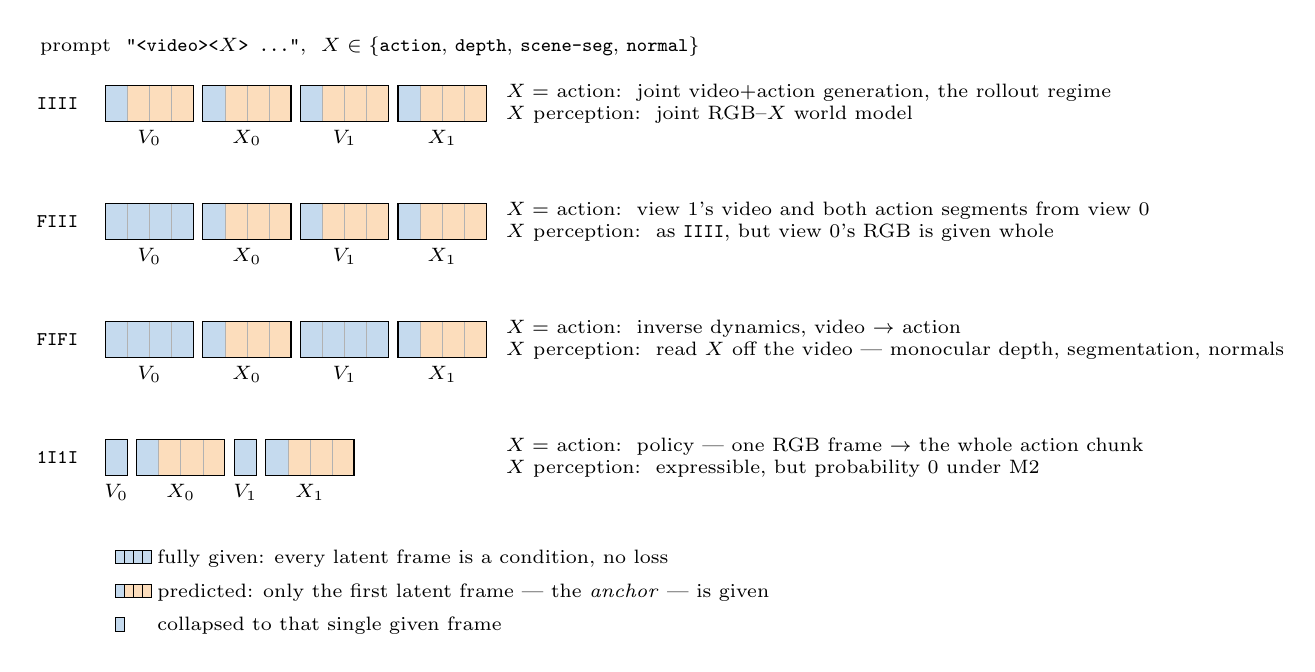
\begin{tikzpicture}[font=\small,
    plan/.style={font=\scriptsize\ttfamily, anchor=east},
    desc/.style={font=\scriptsize, anchor=west, align=left, inner sep=1pt}]

\node[font=\scriptsize, anchor=west] at (-0.95,0.95)
  {prompt \ \texttt{"<video><$X$> \ldots"}, \ $X\in\{$\texttt{action}, \texttt{depth},
   \texttt{scene-seg}, \texttt{normal}$\}$};

% ---- IIII
\node[plan] at (-0.22,0.23) {IIII};
\segI{0}{0}{$V_0$}  \segI{1.24}{0}{$X_0$}  \segI{2.48}{0}{$V_1$}  \segI{3.72}{0}{$X_1$}
\node[desc] at (5.05,0.23)
  {$X=$ action:\ \ joint video+action generation, the rollout regime\\
   $X$ perception:\ \ joint RGB--$X$ world model};

% ---- FIII
\node[plan] at (-0.22,-1.27) {FIII};
\segF{0}{-1.50}{$V_0$}  \segI{1.24}{-1.50}{$X_0$}
\segI{2.48}{-1.50}{$V_1$}  \segI{3.72}{-1.50}{$X_1$}
\node[desc] at (5.05,-1.27)
  {$X=$ action:\ \ view 1's video and both action segments from view 0\\
   $X$ perception:\ \ as \texttt{IIII}, but view 0's RGB is given whole};

% ---- FIFI
\node[plan] at (-0.22,-2.77) {FIFI};
\segF{0}{-3.00}{$V_0$}  \segI{1.24}{-3.00}{$X_0$}
\segF{2.48}{-3.00}{$V_1$}  \segI{3.72}{-3.00}{$X_1$}
\node[desc] at (5.05,-2.77)
  {$X=$ action:\ \ inverse dynamics, video $\to$ action\\
   $X$ perception:\ \ read $X$ off the video --- monocular depth, segmentation, normals};

% ---- 1I1I: one plan only, because under M2 the perception family never draws it
\node[plan] at (-0.22,-4.27) {1I1I};
\segOne{0}{-4.50}{$V_0$}  \segI{0.40}{-4.50}{$X_0$}
\segOne{1.64}{-4.50}{$V_1$}  \segI{2.04}{-4.50}{$X_1$}
\node[desc] at (5.05,-4.27)
  {$X=$ action:\ \ policy --- one RGB frame $\to$ the whole action chunk\\
   $X$ perception:\ \ expressible, but probability $0$ under M2};

% ---- legend
\node[anchor=west] at (0,-5.55) {\anchF};
\node[desc] at (0.62,-5.55) {fully given: every latent frame is a condition, no loss};
\node[anchor=west] at (0,-5.98) {\anchI};
\node[desc] at (0.62,-5.98) {predicted: only the first latent frame --- the \emph{anchor} --- is given};
\node[anchor=west] at (0,-6.41) {\anchOne};
\node[desc] at (0.62,-6.41) {collapsed to that single given frame};
\end{tikzpicture}}
\end{center}
\caption{Every conditioning plan the mixture draws, and what each one means in the two template
families. Each segment is drawn as its strip of latent frames, because that is where the
conditioning lives: a predicted segment still receives its \emph{first} latent frame clean, as an
anchor, and only the rest is denoised. The mask is a property of \emph{positions}, not of
contents, so one diagram per plan covers all four auxiliary streams --- only the task it names
changes, which is the content of the $(\Pi,\sG)$ factorisation. The last row also shows that
segments need not share a length: under \texttt{1I1I} each visual segment collapses to its single
anchor frame while the other stream keeps full length.}
\label{fig:layout}
\end{figure}

\subsection{The training mixture}
\label{sec:mixture}

A step draws a template, then a plan, then builds the sample (\figref{fig:layout}). Our headline
arm uses
\begin{equation}
\begin{split}
\Pi \sim \big[\ &\tmpl{video+action}\!:\!0.4,\quad \tmpl{video+depth}\!:\!0.2,\\
                &\tmpl{video+segmentation}\!:\!0.2,\quad \tmpl{video+normal}\!:\!0.2\ \big].
\end{split}
\label{eq:mix}
\end{equation}
The plan distribution is conditioned on whether $\Pi$ contains an action. For action-bearing
templates we transcribe the upstream distribution decision-for-decision, so the baseline stays
reproducible; the realised marginals are \texttt{IIII} $72.9\%$, \texttt{1I1I} (policy) $9\%$,
\texttt{FIII} $4.05\%$, \texttt{FIFI} $4.05\%$ and video-only $10\%$ (\appref{app:mixture}).

For perception templates the plan distribution is a free parameter, and we argue an important one.
The obvious choice, $\mathrm{M0} = (\texttt{IIII}\,0.10,\ \texttt{FIII}\,0,\ \texttt{FIFI}\,0.90)$,
gives the RGB in full almost always, so the auxiliary modality must be \emph{read off} the video
rather than hallucinated; it is what makes \tmpl{video+depth} an honest depth estimator. We
nonetheless default to $\mathrm{M2} = (0.90,\,0.05,\,0.05)$, matching the action-bearing split, for
two reasons. \emph{(a) Template identity should not predict conditioning level.} Under M0,
\ptag{depth} in the prompt implies ``the RGB will be given'', so the model can read the
conditioning pattern off the tag --- a shortcut that transfers nowhere. \emph{(b) Deployment runs}
\texttt{IIII}. The closed-loop rollout generates \tmpl{video+action} from first frames only, so an
auxiliary stream trained $90\%$ under \texttt{FIFI} learns a discriminative RGB$\to$depth map in a
regime the deployed model never enters. \Secref{sec:modegrid} measures the price of this choice,
which is real.

\subsection{Consistency by construction}
\label{sec:invariants}

Prompt-switched multitask training has a characteristic failure mode: a sample silently becomes a
different task than the mixture specification claims, and every instrument stays green, because
\eqref{eq:loss} is a plain MSE against whatever target was actually built. Three invariants, each
corresponding to a failure we hit.

\textbf{Prompt and layout are decided together.} Upstream decides action dropout inside the forward
pass, by testing whether the action tensor happens to be all zeros. We move that decision into the
dataset, where the prompt is built; otherwise the text promises \ptag{action} for a sequence
containing none. The same rule makes a dataset that cannot serve a requested template fail at
\emph{startup} rather than quietly serve a shorter one.

\textbf{Ground truth comes from the same window and views as the RGB.} View directories are
enumerated by an unsorted glob and two of four are sampled per sample, so re-deriving the mapping
afterwards yields a different draw. The sampled frame indices and view directories are first-class
fields of the sample, which makes it structurally true --- not merely checked --- that a depth
segment and an RGB segment of one view are the same scene, camera and instants.

\textbf{Annotation gaps are startup errors, not training-time degradations.} When $70\%$ of
episodes lacked segmentation targets, a nominal $60/20/20$ action/depth/seg mixture silently
realised as $60/20/6/14$, the last $14\%$ being video-only samples carrying \emph{neither} action
nor perception supervision. A second incident painted $5.2\%$ of all pixels with a reserved colour
that must never occur in training data (\appref{app:incidents}). Both are now startup gates. We
report them not as engineering trivia: in a mixture-of-tasks study, a silent $14\%$ shift in the
realised mixture is larger than any effect we are trying to measure.

\section{Experiments}
\label{sec:exp}

\subsection{Setup}
\label{sec:setup}

\textbf{Data.} A self-generated RLBench \citep{james2020rlbench} tree at $512^2$ with
Colosseum-style domain randomisation \citep{pumacay2024colosseum} over camera pose, table colour
and texture, background texture and light colour: 16 tasks, 4 views, per-frame metric depth and
handle masks. The split is \emph{by variation}: variation-0 (788 episodes) is trained on and all
other variations are held out as unseen task configurations. Windows are 41 frames at stride 3
($6.0$\,s of motion at $6.7$\,Hz); two of four views are sampled per sample.

\textbf{Training.} All arms warm-start from the released Action Images checkpoint (step
125{,}750) and are otherwise identical --- same seed, step count, learning rate, data tree and
prompt style --- so any difference is attributable to the task menu. Full-parameter fine-tuning of
the 5B DiT with ZeRO-2 and CPU-offloaded Adam, bf16, batch size 1 per device on 2 GPUs, learning
rate $5\times10^{-7}$, 1000 warmup steps, constant schedule. Arms: \textbf{arm0}
\tmpl{video+action@1.0} (control), \textbf{arm4} $0.6/0.4$ action/depth, \textbf{arm1}
$0.6/0.2/0.2$ action/depth/segmentation, and the headline \textbf{arm6} of \eqref{eq:mix}.

\textbf{Metrics.} AbsRel for depth, macro-mIoU over the roles present for segmentation, mean
cosine for normals, and for action the median position and geodesic rotation error of the decoded
trajectory. We also report $r_{\text{peak}}$, the per-frame maximum of the red channel: a liveness
signal the loss does not provide, since a low $r_{\text{peak}}$ means the model has stopped drawing
a decodable blob at all. Closed-loop is task success under receding-horizon replanning.

\subsection{One checkpoint, four prompts}

\begin{table}[t]
\caption{Four modalities from one arm6 checkpoint (step 1500), switched by prompt tag alone. Each
row is a separate generation from the same weights on the same held-in episode
(\texttt{open\_drawer}, view 0). $n{=}1$ episode; \tabref{tab:crosstask} gives the cross-episode
spread.}
\label{tab:versatility}
\begin{center}\small
\begin{tabular}{llccc}
\toprule
\textbf{Prompt} & \textbf{Metric} & \texttt{IIII} & \texttt{FIII} & \texttt{FIFI} \\
\midrule
\ptag{video}\ptag{action}    & $r_{\text{peak}}\uparrow$ (of 255) & 252.9 & 252.8 & 252.1 \\
\ptag{video}\ptag{depth}     & AbsRel $\downarrow$   & \best{0.087} & 0.059 & 0.652 \\
\ptag{video}\ptag{scene-seg} & macro-mIoU $\uparrow$ & \best{0.386} & 0.354 & 0.343 \\
\ptag{video}\ptag{normal}    & mean $\cos\uparrow$   & 0.896 & 0.919 & \best{0.937} \\
\ptag{video}                 & PSNR (dB) $\uparrow$  & 16.8 & 30.7$^\dagger$ & n/a$^\ddagger$ \\
\bottomrule
\multicolumn{5}{l}{\scriptsize $^\dagger$ segment is fully given; the value is the VAE round-trip, not a prediction.}\\
\multicolumn{5}{l}{\scriptsize $^\ddagger$ video is its own anchor, so \texttt{FIFI} would violate \eqref{eq:nonempty}.}
\end{tabular}
\end{center}
\end{table}

\tabref{tab:versatility} is the central versatility result: 1500 steps (${\approx}1\%$ of the
original training budget) suffice for one checkpoint to answer four different questions about the
same scene, selected by four different prompts, with the same weights and the same head. Depth is
decodable to $8.7\%$ AbsRel \emph{while the RGB it must be consistent with is itself being
predicted}; normals reach $0.90$--$0.94$ cosine against a VAE ceiling of $0.99$; nine-way dense
role segmentation reaches $0.39$ macro-mIoU; and the action stream keeps
$r_{\text{peak}}\approx253$ with zero weak frames, i.e.\ the policy is intact. A second arm
confirms the pattern is not mixture-specific: arm1 at step 2000 gives, under \texttt{IIII} over
both views, depth AbsRel $0.088/0.114$ and segmentation macro-mIoU $0.426/0.566$.

\subsection{The conditioning axis is not free}
\label{sec:modegrid}

\begin{table}[t]
\caption{Depth across four held-in episodes at arm6 step 4500. \texttt{FIFI} --- the ``easy''
discriminative mode, where both RGB views are given in full --- receives $5\%$ of perception
probability mass under M2, and it is the mode that fails, on some episodes only. \texttt{IIII}, the
deployment regime, is stable everywhere.}
\label{tab:crosstask}
\begin{center}\small
\begin{tabular}{lcccc}
\toprule
\textbf{Episode} & \texttt{IIII} AbsRel $\downarrow$ & \texttt{FIII} AbsRel $\downarrow$ & \texttt{FIFI} AbsRel $\downarrow$ & given-RGB PSNR \\
\midrule
\texttt{open\_drawer}  & 0.160 & 0.069 & \textcolor{red!70!black}{1.335} & 30.7 \\
\texttt{push\_buttons} & 0.065 & 0.103 & \best{0.041} & 38.2 \\
\texttt{stack\_wine}   & 0.116 & 0.106 & 0.123 & 31.5 \\
\texttt{turn\_tap}     & 0.059 & 0.029 & \best{0.035} & 34.6 \\
\midrule
mean & 0.100 & 0.077 & 0.384 & --- \\
\bottomrule
\end{tabular}
\end{center}
\end{table}

\tabref{tab:crosstask} isolates the cost of the M2 plan distribution. Under \texttt{IIII} ---
$90\%$ of perception draws, and the regime the policy is deployed in --- depth is stable across
episodes ($0.059$--$0.160$) and across training ($0.087$ at step 1500, $0.086$ at 3500, $0.085$ at
4000). Under \texttt{FIFI}, which receives $5\%$ of the mass, the same checkpoint gives AbsRel
$1.34$ on \texttt{open\_drawer} and $0.04$ on \texttt{push\_buttons}: the under-trained mode has
become episode-dependent, and on the one episode we track through training it degrades
monotonically ($0.652 \to 1.167 \to 1.335$), while \texttt{FIII} oscillates instead ($0.059$,
$1.303$, $0.069$), which reads as instability rather than forgetting (\appref{app:overtraining}).
Segmentation moves the other way over the same interval ($0.386 \to 0.449$ under \texttt{IIII}).

This is the central trade of the framework. The plan distribution is not a hyperparameter that
only affects convergence speed; it decides \emph{which questions the finished checkpoint can still
answer}. M0 buys a strong depth estimator and a weak world model, M2 the opposite. A mixture that
wants both must pay for both, and on 788 episodes we could not.

\subsection{The policy survives, and keeps its modes}

\begin{table}[t]
\caption{Action quality of the four-stream checkpoint (arm6, step 4500) under every action-bearing
mode it was trained on, decoded to 6-DoF poses (\texttt{open\_drawer}, view 0, $n{=}1$ episode).
More given video yields better action, which is the ordering the conditioning axis predicts.}
\label{tab:action}
\begin{center}\small
\begin{tabular}{lccccc}
\toprule
\textbf{Mode} & pos.\ err.\ med.\ (cm) $\downarrow$ & pos.\ err.\ mean (cm) $\downarrow$ & rot.\ err.\ med.\ ($^\circ$) $\downarrow$ & frac.\ ${>}90^\circ$ $\downarrow$ & $r_{\text{peak}}\uparrow$ \\
\midrule
\texttt{FIFI}   & \best{1.9} & \best{2.3} & \best{18.7} & 0.049 & 250.8 \\
\texttt{FIII}   & 4.5 & 7.4 & 19.8 & 0.049 & 252.4 \\
\texttt{IIII}   & 5.4 & 6.4 & 20.9 & 0.049 & \best{254.1} \\
\texttt{policy} & 14.8 & 14.5 & 26.9 & 0.268 & 251.0 \\
\bottomrule
\end{tabular}
\end{center}
\end{table}

\tabref{tab:action} shows the four-stream checkpoint still produces usable trajectories under every
action-bearing mode. The ordering is exactly the information ordering --- \texttt{FIFI} sees both
videos in full and solves an inverse-dynamics problem, \texttt{IIII} must invent the future it acts
in, and \texttt{policy} sees a single frame --- which is a sanity check that the conditioning axis
does what it claims. That a checkpoint whose training mixture is $60\%$ non-action still recovers
$1.9$\,cm inverse dynamics is our strongest evidence that the shared head is not being torn apart
by the auxiliary streams.

\subsection{Closed-loop success, and what the loss does not tell you}

\begin{table}[t]
\caption{Closed-loop success on 5 RLBench tasks, $n{=}20$ scenes each ($n{=}100$ total), paired by
scene seed, McNemar per task. ``official'' is the shared warm-start checkpoint, so each column is
the net effect of fine-tuning \emph{relative to its own initialisation}, not an external baseline.
The fine-tuned arm is in-domain and the official checkpoint is zero-shot on this rig; this is a
home-advantage comparison, not a model ranking.}
\label{tab:closedloop}
\begin{center}\small
\begin{tabular}{lccccc}
\toprule
\textbf{Task} & official (init) & arm4 @5k & arm4 @10k & McNemar $b/c$ & $p$ \\
\midrule
\texttt{close\_box}       & \best{80\%} & 70\% & 60\% & 3/5 & 0.727 \\
\texttt{close\_drawer}    & 5\%  & 45\% & \best{80\%} & 8/0 & \best{0.0078} \\
\texttt{push\_buttons}    & 5\%  & \best{40\%} & 20\% & 8/1 & \best{0.039} \\
\texttt{meat\_off\_grill} & 10\% & 0\%  & 15\% & 0/2 & 0.500 \\
\texttt{open\_drawer}     & 0\%  & 0\%  & 0\%  & 0/0 & 1.000 \\
\midrule
\textbf{total} & 20\% & 31\% & \best{35\%} & 19/8 & 0.052 \\
\bottomrule
\end{tabular}
\end{center}
\end{table}

\tabref{tab:closedloop} reports closed-loop success for the depth co-training arm. Two tasks
improve significantly over the initialisation ($+40$ and $+35$\,pp, both $p<0.05$), two move the
other way without significance, and the pooled effect sits exactly on the threshold ($p=0.052$,
$95\%$ CI $[+1,+21]$\,pp). We report it that way rather than rounding: per-task effects of opposite
sign cancel, and reporting only ``$31\%$ vs $20\%$'' would hide both real effects. The action-only
control (arm0) is flat from step 750 to 2500 ($20$--$30\%$, overlapping confidence intervals).

\textbf{Loss does not order checkpoints.} At step 7500, arm4's success falls to $6.7\%$ ($n{=}60$)
from $28.8\%$ at 2500 and $36.7\%$ at 10000 (Fisher $p=1.0\times10^{-4}$ against 10000), and the
collapse is present on every task, not one. Over the same interval the training loss is at its
\emph{lowest} of the whole run (mean $0.0486$ over steps 7000--7500 and $0.0457$ over 7500--8000,
versus $0.0487$ immediately before), with no outlier steps. A transient exists that costs $5\times$
the success rate and then recovers on its own, and the diffusion objective is completely blind to
it. Practically: checkpoint selection by loss is invalid here, dense checkpointing plus rollout
evaluation is mandatory, and any single-step comparison between two arms is untrustworthy.

\section{Limitations}
\label{sec:limitations}

\textbf{Scale.} 788 training episodes, 16 simulated tasks, a single seed.
\citet{zhuang2025argus} report accuracy loss on \emph{every} task once a multitask vision model's
task set outgrows its data, and we sit three orders of magnitude below their data budget --- which
is why our headline arm caps the auxiliary set at three streams. We cannot separate ``four streams
is the right number'' from ``four streams is what 788 episodes can carry''.

\textbf{Evaluation breadth.} The modality tables are $n{=}1$ episode for three of the four streams
and $n{=}4$ for depth, on \emph{held-in} variation-0 scenes; the 478 held-out episodes have not
been swept. \tabref{tab:closedloop} is $n{=}100$ paired scenes but measures the action/depth arm,
not the four-stream arm, whose training had reached step 4500 of a planned 10000.

\textbf{The tag is not isolated from the anchor.} Every mode we evaluate gives the target segment
its first latent frame as a clean anchor, which is itself an instance of the requested modality.
The prompt tag and the anchor therefore always agree, and we have not established how much of the
modality selection each one carries. Isolating that requires training-time exposure to tag-only
conditioning, which the current mixture does not contain.

\textbf{One gate is not measured.} The action stream's codec floor ($\approx4$\,mm 3D) is known,
but its VAE round-trip is not: unlike the perception streams, the action canvas is rendered inside
the forward pass from the trajectory and both cameras rather than loaded from disk, so measuring it
needs a harness that re-renders, round-trips and then re-runs the multi-view pose fusion, which the
three perception gates do not share. We report that cell as unmeasured rather than inferring it
from the RGB control.

\textbf{Untrained cells, and simulation only.} \Eqref{eq:layout} expresses three-modality templates
and substitution templates such as $[\,D_0\mid A_0\mid D_1\mid A_1\,]$; neither is trained here,
and both are stated as reachable structure rather than as results. Depth and role masks are
simulator ground truth, so extending to real data means pseudo-labels --- and our own probing found
monocular pseudo-depth on in-the-wild robot video to lack the metric anchor that
\eqref{eq:depthcodec} requires.

\section{Conclusion}

A world action model can co-generate action, depth, dense semantic roles and surface normals
through a single shared output head, with the modality selected by a prompt tag and the task type
--- perception versus world model --- selected by an orthogonal conditioning mask. The construction
costs no new parameters and, for two-modality templates, no extra compute, because an auxiliary
modality occupies the slot the action would have used. The $(\Pi,\sG)$ factorisation is what makes
claims in this area falsifiable: it separates a depth-space world model from monocular depth
estimation, and it exposes the conditioning mixture as a design decision that determines which
questions a finished checkpoint can still answer. That point, together with the finding that
diffusion loss does not order checkpoints by closed-loop success, is what we would most want a
reader building in this direction to take away.

\subsubsection*{Reproducibility Statement}
All arms are launched by a single script parameterised only by the template mixture; the data tree,
seed, step count, learning rate, warm-start checkpoint and prompt style are held fixed across arms
and stamped into the output path, so that two differently-configured runs cannot share a directory.
The codec admission gate, the mixture probabilities, the exact command lines, and the artifact from
which each reported number was extracted are given in the appendix and in the code release.

\bibliography{reference}
\bibliographystyle{iclr}

\appendix

\section{Codec details}
\label{app:codecs}

\paragraph{Depth.}
The RGB-cube path of \eqref{eq:depthcodec} visits black, red, yellow, green, cyan, blue, magenta,
white --- eight vertices and seven unit edges, one coordinate flipping per step. Encoding clips to
a sanity range of $0.05$--$10$\,m and writes an off-path sentinel $(128,0,128)$ outside it.
Decoding solves
\begin{equation}
(k^\star,\alpha^\star) \;=\; \arg\min_{k\in\{0,\dots,6\},\,\alpha\in[0,1]}
\big\|\vgamma - \big((1-\alpha)\vv_k+\alpha\vv_{k+1}\big)\big\|^2 ,
\qquad \hat y = \tfrac17\big(k^\star+\alpha^\star\big),
\label{eq:depthdecode}
\end{equation}
and inverts the transform as $\hat d = \lambda c\,\big(1-(1-\hat y)^{1/(\lambda+1)}\big)$. Any pixel whose
residual in \eqref{eq:depthdecode} exceeds a threshold is reported as invalid rather than returned
as a plausible depth.

\paragraph{Surface normal.}
In a right-handed camera frame with pinhole focal lengths $(f_x,f_y)$ in pixels,
\begin{equation}
\vn \;\propto\; \left(-\frac{f_x}{z}\frac{\partial z}{\partial u},\;
-\frac{f_y}{z}\frac{\partial z}{\partial v},\; 1\right)^{\!\top},
\qquad \text{stored as } \tfrac12(\vn+1),
\label{eq:normal}
\end{equation}
following the visualisation convention of \citet{zhuang2025argus}. The $f/z$ factors are not
optional: taking $\nabla z$ in pixel units, as an earlier version of our own code did, is wrong by
$f_x/z \approx 200$--$750$ on this data and flattens every surface systematically toward the
camera --- while producing entirely plausible-looking normal maps. Derivatives are central
differences, one-sided at the border. We deliberately emit \emph{no} invalid sentinel: the
simulator renders sky at a constant far-clip depth that \eqref{eq:depthcodec} already encodes as an
ordinary surface, and a constant-depth region has zero gradient, hence maps to $(0,0,1)$, a
camera-facing plane. The two streams must not disagree about what the sky is.

\paragraph{Segmentation.}
Nine roles with globally fixed colours: \texttt{background} (black), \texttt{target} (red),
\texttt{goal} (green), \texttt{robot\_arm} (blue), \texttt{gripper} (cyan), \texttt{distractor}
(yellow), \texttt{tool} (magenta), \texttt{fixture} (purple), \texttt{unknown} (orange). Two
constants are calibrated rather than chosen: the role$\,\to\,$colour assignment is permuted so that
the tightest pair in sRGB distance ($98.3$) lands on \texttt{unknown}, a class that must never occur
in valid data, and the background gate $\tau = 40$ is set against that measured minimum rather than
a nominal one. Encoding is a handle$\,\to\,$role$\,\to\,$colour lookup, so roles cannot overlap and
there is no paint order to get wrong; decoding is nearest-colour classification restricted to the
roles the episode can legally contain, and uses \emph{no} connected-component pruning: the standard instance-decode
post-processing deletes legitimate few-pixel targets outright (e.g.\ \texttt{sweep\_to\_dustpan}'s
dirt, five handles of 4--8\,px). A handle's role is its instruction-independent base role, then
promotion to \texttt{target} for handles the instruction refers to \emph{and} whose base role is a
manipulable object --- a referred receptacle stays a \texttt{goal} and a referred implement stays a
\texttt{tool}, since 9 of the 16 tasks name two or three objects in a single instruction.

\section{Realised mixture probabilities}
\label{app:mixture}

For an action-bearing template draw (upstream values, transcribed decision-for-decision):
\begin{center}\small
\begin{tabular}{llr}
\toprule
\textbf{Outcome} & \textbf{Composition} & \textbf{Probability} \\
\midrule
video-only (action dropout)           & $0.10$ & $10.0\%$ \\
\texttt{policy} (single-frame visual) & $0.90\times0.10$ & $9.0\%$ \\
\texttt{IIII} & $0.90\times0.90\times0.90$ & $72.9\%$ \\
\texttt{FIII} & $0.90\times0.90\times0.05$ & $4.05\%$ \\
\texttt{FIFI} & $0.90\times0.90\times0.05$ & $4.05\%$ \\
\bottomrule
\end{tabular}
\end{center}
For perception templates the presets over
$(\texttt{IIII},\ \texttt{FIII},\ \texttt{FIFI},\ \text{single-frame anchor})$ are
$\mathrm{M0}=(0.10,0,0.90,0)$, $\mathrm{M1}=(0.45,0.10,0.45,0)$ and
$\mathrm{M2}=(0.90,0.05,0.05,0)$; all experiments here use M2. The single-frame branch means
something different for the two families: with an action present, collapsing every visual segment
still leaves the action segments to predict, whereas in an all-visual template collapsing
everything would violate \eqref{eq:nonempty}, so only the anchor is collapsed.

\section{Auxiliary streams over training}
\label{app:overtraining}

\begin{center}\small
\begin{tabular}{lccccc}
\toprule
\textbf{Step} & depth \texttt{IIII} $\downarrow$ & depth \texttt{FIII} $\downarrow$ & depth \texttt{FIFI} $\downarrow$ & seg \texttt{IIII} $\uparrow$ & seg \texttt{FIFI} $\uparrow$ \\
\midrule
1500 & 0.087 & 0.059 & 0.652 & 0.386 & 0.343 \\
3500 & 0.086 & --- & --- & --- & --- \\
4000 & 0.085 & 1.303 & 1.167 & \best{0.449} & \best{0.592} \\
4500 & 0.160 & 0.069 & 1.335 & --- & --- \\
\bottomrule
\end{tabular}
\end{center}
arm6, \texttt{open\_drawer}, view 0. Depth under the deployment regime \texttt{IIII} is flat,
segmentation improves, and the low-probability \texttt{FIFI} depth mode degrades. The training loss
over the same interval is smooth and predicts none of it.

\section{Two silent-failure incidents}
\label{app:incidents}

\textbf{Realised-mixture drift.} \texttt{seg\_targets.json} is generated offline, so every episode
added by the scene generator arrives without it. An episode with no segmentation target resolves
nothing, at which point the sample drops \texttt{segmentation} from its template and silently
becomes a plain \tmpl{video} one. Measured over the tree at the time, $70\%$ of variation-0
episodes were affected ($97\%$ of the newly generated ones), turning a nominal $60/20/20$
action/depth/seg mixture into roughly $60/20/6/14$ --- where the final $14\%$ carried neither
action nor perception supervision. The loss curve was normal throughout, the construction-time
self-test passed (it probes episodes until one works), and the run's own logs reported whatever
mixture was on the command line. The loader now refuses to start above a $10\%$ miss rate.

\textbf{An unmapped handle in the segmentation target.} The simulator renders ``no object'' (the
sky above the room walls) as $-1$, which the mask writer converts to $\mathtt{0xFFFFFF}$ and then
truncates to $\mathtt{0xFFFF}$ on the cast to \texttt{uint16}. That value reached the
handle$\,\to\,$role lookup unmapped and was painted with the reserved \texttt{unknown} colour:
$5.2\%$ of all pixels over 11{,}200 frames, up to $52.9\%$ in a single view. Nothing flagged it,
because \eqref{eq:loss} is a plain MSE against whatever target was built, and the one test that
did check pointed at a data root whose symlink had gone stale. A startup probe over a spread of
episodes now checks it and cannot be skipped.

\section{Number provenance}

Every number in this paper is extracted from a stored artifact rather than transcribed from a log;
the mapping from table cell to artifact path is listed in \texttt{paper/README.md} in the code
release. The modality grid comes from a single script that loads the checkpoint once and sweeps
every (template, mode) pair, recomputing segment spans from the same rule the inference path uses
and asserting the total against the array actually returned, so that a slicing disagreement cannot
silently move a metric onto the wrong pixels.

\end{document}
